
Next, we propose two new variability-aware job scheduling policies, the \textit{Power
Ratio Variability Prediction} and the \textit{Variability-Trained Prediction}. These
schedulers make use of the power variability prediction models introduced in Section
~\ref{sec:variability_prediction}. With these models, the schedulers predict the job's
power consumption on all available sockets and schedule the job on the most efficient one.
Before scheduling the job, the scheduler checks whether the system wide power budget would
be respected once the job starts running. If this is not the case, the job will wait until
other jobs finish and more power is available. In the case of multi-node jobs, we consider 
the total power consumption of all its processes.  If possible, sockets on the same node
are preferred, but intra-node topology is not considered.  
Furthermore, we consider three job scheduling policies representative of the
state-of-the-art and with increasing complexity: \textit{SLURM extended}, \textit{Power
Estimation}, and \textit{Power Estimation+Variability Aware}.  The first two are
variability-agnostic, while the third is variability-aware.  Finally, we also consider an
\textit{Ideal Variability Prediction}, which is based on an oracle power variability
predictor that knows exactly how much power a job will consume on any processor in the
system.  We extend the SLURM's logic~\cite{slurm_02} to implement the various power- and
variability-aware job scheduling policies presented in this section. We chose SLURM as our
reference because it is widely used on HPC production systems and well studied in the
literature.  All job scheduling policies are described in the following:
\par
\textit{SLURM Extended}: This policy implements SLURM scheduler's logic.  We extend the
default behavior to not exceed the global power budget, by considering the worst case
scenario, which is that each job can consume the maximum power budget allowed per socket.
Additionally, we extend the scheduler to initiate backfilling for power as
well~\cite{Patki:2015:PRM:2749246.2749262}.  Traditionally, if a job requests more sockets
than currently available, the scheduler will try to schedule a different job without
causing delays.  The same will happen if a job requests more power than the system can
allocate.
\par
\textit{Power Estimation} (\PESched): This policy extends further \DefaultSched's behavior
by using a user provided estimation of a job's power consumption.  For precision we obtain
power profiles of previous execution of the jobs to estimate the power consumption.  This
is the equivalent of using a variability-agnostic prediction model.  This scheduler does
not consider manufacturing variability as it assumes all sockets consume the same power
for a given job.
\par
\textit{Power Estimation+Variability Aware} (\PEVASched): This policy implements elements
from the state-of-the-art practices in power-aware job
scheduling~\cite{Gholkar:2016:PTH:2967938.2967961,Inadomi:2015:AMI:2807591.2807638}.
Similarly to \PESched, it estimates the power requirements of a job using a power trace
from a previous execution, same as \PESched.  It also orders sockets and allocates first
the most power efficient ones to minimize the system's net power consumption.  The socket
ordering is obtained by running a simple benchmark, the \textit{cholesky} kernel, on all
sockets and observing their power consumption.  A drawback of this approach is that it
assumes all parallel jobs to be influenced by manufacturing variability in the very same
way.  Another drawback is that a job's power estimation depends on the socket used for
profiling and thus it is possible to under or over-estimate the final power.

\begin{figure}[!t]
	\centering
        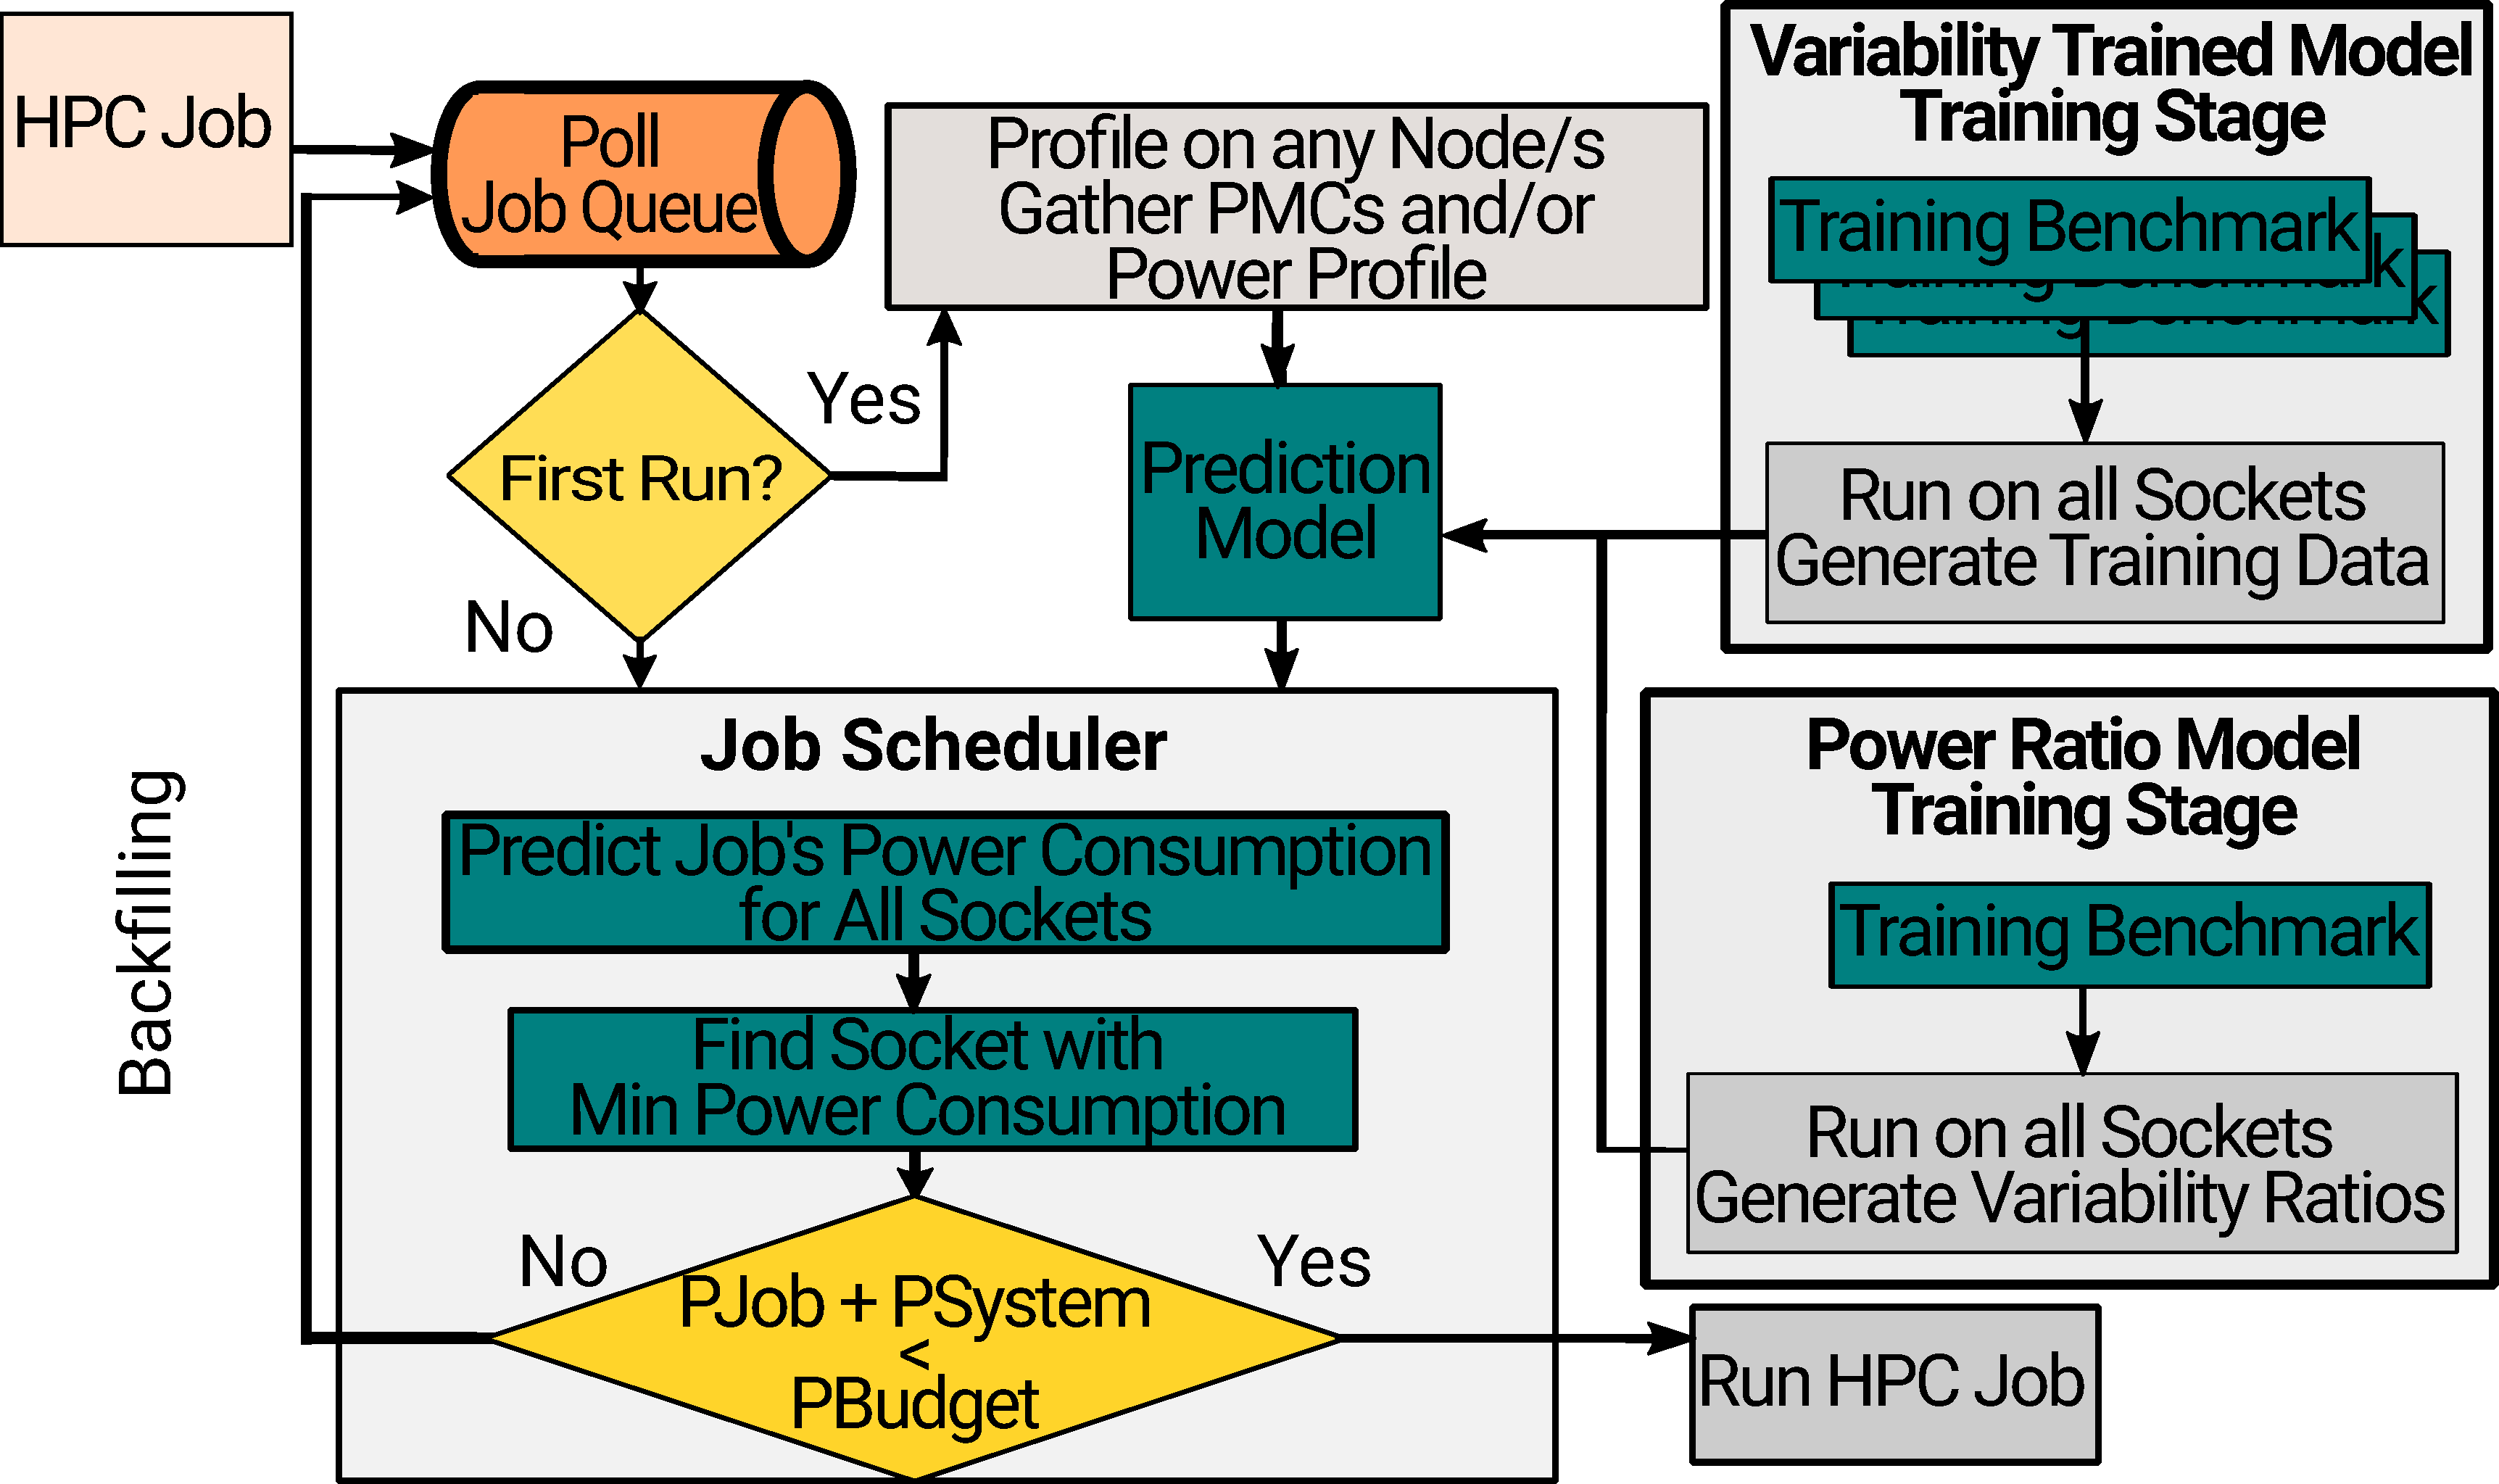
\includegraphics[width=.8\textwidth]{power_aware_job_scheduling/figures/pred_policy_recipe}
        \caption{Framework for the \PRVSSched~ and \PMCVSSched. The upper right box shows the steps for training the PMC model, while Power Ratio training stage is shown in the box below.  }
        \label{fig:pred_policy_recipe}
\end{figure}

\par
\textit{Power Ratio Variability Prediction} (\PRVSSched):  This is the first new policy we
propose.  It relies on our Power Ratio Model, presented in Section~\ref{sec:naive_model},
to guide scheduling decisions.  A single power and performance profile of a given job (or
one for each socket a process was run on, in the case of multi-node jobs) is required in
order to compute the activity ratios, which can be performed on any set of sockets in the
system.  Running the single benchmark a priori on all sockets is also required. 
\par
If the predicted power for a new job makes the system budget to go over its limit, then
the job waits until resources are released.  The backfilling scheme is the same as with
the previous policies.  This policy's framework is shown in
Figure~\ref{fig:pred_policy_recipe}.  Note that two training processes are shown in the
figure, for the different power prediction models proposed in this work.  The lower box
shows corresponds to the \PRVSSched~ policy.
\par
\textit{Variability-Trained Prediction} (\PMCVSSched): Our second proposed policy is
similar to the PRVS policy, but it uses our VT prediction model, presented in
Section~\ref{sec:pmcs_model}, to obtain power consumption  predictions.
%\footnote{The \textit{Generic PMC} model is not used due to its poor prediction
%capabilities, which are shown in Section~\ref{sec:model_validation}.} 
This policy requires running the training benchmark set from Table~\ref{tab:training_set}
on all sockets in order to train the model.  Using the variability aware power
predictions, scheduling decisions are made in the same manner as with the \PRVSSched~
approach.  The framework for this policy is described in
Figure~\ref{fig:pred_policy_recipe}.  The box on the upper right corner corresponds to the
training process of the \textit{PMC-based Prediction Models}, used by \PMCVSSched.
\par
\textit{Ideal Variability Prediction} (\IVSSched): Identical to \PRVSSched~ and
\PMCVSSched, but using an oracle power predictor to drive job scheduling decisions.  This
policy is aimed at showing the impact of using a 100\% accurate model to guide scheduling
decisions. Thus, \IVSSched~ is used for comparison purposes to show the maximum benefits
that can be achieved by power- and variability-aware job scheduling policies.

